% ======================================================== 
% DEV1 - Développement I (Algorithmique et langage Java)
% HE2B - ESI
%
% Errata, lorsqu'il faut ajouter un errata
%
%                                     Marco Codutti
%                                     Pierre Bettens
% ======================================================== 

\documentclass[a4paper,doubleside,11pt]{book}

%=========================
% Les styles
%=========================
% ===============================================================
%       Feuille de style LaTeX pour un syllabus à l'ESI
% ---------------------------------------------------------------
% On suppose qu'on travaille avec la classe book
%                                                   Marco Codutti
% ===============================================================


% ===================================================
%   Style commun à tout type de document
% ===================================================
% ===============================================================
%   Partie commune à tout type de document : 
%		syllabus, td, interro...
% ===============================================================

\usepackage[utf8]{inputenc}     % Source en UTF8, permet les accents
\usepackage[T1]{fontenc}        % Permet les accents dans le PDF
\usepackage[francais]{babel}    % Gestion du français
\usepackage{textcomp}	        % Plein de symboles
\usepackage{lmodern}            % Police de caractères moderne
\usepackage[
	hmargin=3.5cm,
	vmargin=3cm
	]{geometry} 				% Géométrie de la page
\usepackage{caption}
\usepackage{subcaption}


% ===================================================
%   Style des (sub)sections
% ===================================================

% Permet d'avoir les numéros de (sub)sections dans la marge
% Tiré de "Latex Howtos" de Sébastien Combéfis
% -------------------------------------------------------------
\makeatletter
\def\@seccntformat#1{\protect\makebox[0pt][r]{\csname the#1\endcsname\quad}}
\makeatother


% ===================================================
%   Style des paragraphes
% ===================================================

% Enlever l'indentation de chaque première ligne de paragraphe
% + léger espace entre les paragraphes.
% http://www.ctan.org/pkg/parskip
% -------------------------------------------------------------
\usepackage{parskip}
\raggedbottom

% Pour barrer d'une croix tout un block
% \begin{wrong}\begin{LDA}...\end{LDA}\end{wrong}
\usepackage{environ}
\NewEnviron{wrong}{%
%	\begin{tikzpicture}
%		\node (box){\begin{minipage}{\linewidth}\BODY\end{minipage}};
%		\draw[gray] (box.north west) -- (box.south east); % pour un trait en diagonale principale
%		\draw[gray] (box.south west) -- (box.north east); % pour un autre trait en diagonale 
%	\end{tikzpicture}
	\begin{minipage}{\linewidth-2mm}\BODY\end{minipage}
	\hskip-5mm
	
\includegraphics[width=1cm]{icon/dont}
	}
\NewEnviron{correct}{%
%	\begin{tikzpicture}
%		\node (box){\begin{minipage}{\linewidth}\BODY\end{minipage}};
%		\draw[gray] (box.north west) -- (box.south east); % pour un trait en diagonale principale
%		\draw[gray] (box.south west) -- (box.north east); % pour un autre trait en diagonale 
%	\end{tikzpicture}
	\begin{minipage}{\linewidth-2mm}\BODY\end{minipage}
	\hskip-5mm
	%\includegraphics[width=1cm]{icon/do}
	}
	
% ===================================================
%   Paragraphes spéciaux
% ===================================================

%---------------------------------------
% Citation en début de chapitre
%---------------------------------------
\newenvironment{Exergue}{%
	\begin{quote}
	\itshape
	}{
	\end{quote}
	\vskip2\baselineskip
	}

%---------------------------------------
% \begin{Emphase}...\end{Emphase}
% Met en évidence un ou des paragraphes
% début de cadre en gris
%---------------------------------------
\newenvironment{Emphase}%
  {%
	\par\nobreak%
	\bgroup%
		\color{gray}%
		\hskip-0.3cm%
		\rule{4cm}{0.5pt}%
		\hskip-4cm%
		\rule[-2em]{0.5pt}{2em}%
		\vskip-2.5em%
	\egroup%
  }{%
	\par\nobreak%
	\bgroup%
		\color{gray}%
		\vskip-2em%
		\hskip-0.3cm%
		\rule{0.5pt}{2em}%
		\rule{4cm}{0.5pt}%
		\hskip-4cm%
	\egroup%
  }

%---------------------------------------
% Notes
%---------------------------------------
\usepackage{mdframed}
\newenvironment{Note}{}{}
\surroundwithmdframed[
	skipabove=0.5\baselineskip,
	topline=false,
	leftline=true,
	bottomline=false,
	rightline=false,
	innerrightmargin=0pt,
	innerlinewidth=2pt,
	font=\normalsize,
	linecolor=gray,
	fontcolor=black
]{Note}

%---------------------------------------
% Pour mettre une icone en marge
% Utilisation: \marginicon{nomIcone}
% L'icone doit être présente dans le dossier icon
% dans un format reconnu (pas de gif)
%---------------------------------------
\usepackage{marginnote}
\newcommand{\marginicon}[1]{
	\marginnote{\includegraphics[width=25px]{icon/#1}}[8pt]
}

% ===================================================
%   Style des textes
% ===================================================

% Permet d'avoir des couleurs
% xxxnames pour noms prédéfinis
% table pour colorier toute une table
% http://www.ctan.org/pkg/xcolor
% -------------------------------------------------------------
%\usepackage[usenames,dvipsnames,svgnames]{xcolor}
\usepackage[usenames,dvipsnames,svgnames,table]{xcolor}
\usepackage{colortbl}
\usepackage{makecell}
\setlength{\tabcolsep}{10pt} % Default value: 6pt
\renewcommand{\arraystretch}{1.5} % Default value: 1

% Permet de barrer, souligner, ...
% Pour barrer : \sout{texte}
% -------------------------------------------------------------
%\usepackage[normalem]{ulem}

% subscript facile
% -------------------------------------------------------------
%\newcommand\textsubscript[1]{\ensuremath{{}_{\mathrm{#1}}}}
% commenté car le compilateur indique qu'il est déjà défini

% ===================================================
%   Style des listes en tout genre
% ===================================================

% Un grand contrôle sur l'aspect des listes
% -------------------------------------------------------------
\usepackage{enumitem}
\setdescription{font=\sffamily\bfseries, style=nextline, labelsep=*}
\setlist[itemize]{label=$\triangleright$,leftmargin=8mm,itemsep=1mm}
\setlist[enumerate]{itemsep=1mm}


% ===================================================
%   Style des images
% ===================================================

% Gestion des images.
% http://www.ctan.org/pkg/graphicx
% -------------------------------------------------------------
\usepackage{graphicx}

% Modification du style pour les captions des figures
% Permet \captionof si on ne veut pas de figure
% -------------------------------------------------------------
\usepackage[font=scriptsize,labelfont=sc,skip=5pt]{caption}

% Pour des images entourées de textes.
% -----------------------------------
\usepackage{wrapfig}


% ===================================================
%   Style des tableaux
% ===================================================

\usepackage{array}		% Permet d'utiliser 'm' dans tabular
\usepackage{hhline}		% Permet \hhline pour une ligne double ou partielle

% ===================================================
%   Style pour les math
% ===================================================

\usepackage{mathdots}	% Permet d'avoir un \vdots qui respecte la taille demandée
\usepackage{amsfonts}	% Permet d'avoir des symboles en plus comme \checkmark
\usepackage{amsmath} 	% Pour xrightarrow

% ===================================================
%   Style pour les colonnes
% ===================================================

% Permet d'avoir du texte sur plusieurs colonnes à l'intérieur du document.
\usepackage{multicol}


\usepackage{comment}
% ===================================================
%   Éléments remarquables du document
%   sommaire, toc, index...
% ===================================================
\usepackage{minitoc}
\renewcommand{\mtctitle}{Contenu}

% Sommaire
% La toc complète doit aussi être présente
%-------------------------------------------
\usepackage{shorttoc}

% Index
%--------------
\usepackage{makeidx}
\makeindex

% TOC
%--------------
% décaler à droite chap et section dans toc
\usepackage{tocloft}
\addtolength{\cftchapindent}{1cm}
\addtolength{\cftsecindent}{1cm}
\addtolength{\cftsubsecindent}{1cm}



% ===================================================
%   Style des chapitres
% ===================================================

% Pour un plus beau style pour le titre de chapitre
\usepackage[Lenny]{fncychap}

\usepackage{fancyhdr}
\fancypagestyle{plain}{				% Redéfinir le style plain
	\fancyhf{} 						% Enlever tout
	\fancyhead[RO,LE]{\thepage}
	\renewcommand{\headrulewidth}{0pt} % pas de ligne en entête
}


% ===================================================
%    Numérotation des notes de bas de page
% ===================================================
 
\usepackage{chngcntr} % permet de gérer la numérotation des footnote
\counterwithout{footnote}{chapter} % ne pas recommencer la numérotation 
								   % à chq chapitre
\counterwithout*{footnote}{part}   % ne pas recommencer la numérotation 
                                   % à chaque part

% =============================================
%   Permet d'ajouter des exercices numérotés
%
%	\begin{Exercice}{titre}
%		blabla
%	\end{Exercice}
% =============================================

\usepackage{fancybox}
\usepackage{calc}

% Pour un exercice avec numérotation automatique
\newcounter{exercicenum}
\setcounter{exercicenum}{0}			% Si 0 -> 1er exercice = n°1
\newlength{\widthexercice}

\newenvironment{Exercice}[1]%
{%
	\refstepcounter{exercicenum}	% Incrémenter le compteur
	\settowidth{\widthexercice}{\scriptsize Exercice \normalsize\theexercicenum}
	\subsubsection*{%
		\hspace{-\widthexercice} 				% Décaler le numéro à gauche
		\hspace{-0mm}
		\large%
		{%
			\color{MidnightBlue}%
			\sffamily%
			\Ovalbox{\scriptsize Exercice \normalsize\theexercicenum}	% Le numéro
		}%
		\hspace{1pt}
		{\sffamily\bfseries#1}	% Le titre
	}
	\nopagebreak}{%
}{%
}

% ========================================================
%  Permet d'ajouter des graphiques Tikz (flow charts,...)
% ========================================================

% === Pour faire des dessins via TikZ
\usepackage{tikz}
\usetikzlibrary{matrix}
\usetikzlibrary{shapes.geometric,arrows}
\usetikzlibrary{positioning}

% === Synopsis adaptés aux nombres d'entrées et de sorties

\newcommand{\flowalgo}[1]{
	\begin{tikzpicture}
	\sffamily
	\matrix [column sep = 2em] {
		\node[draw, rounded corners, thick] (M) {#1};\\
	};
	\end{tikzpicture}
}

\newcommand{\flowalgor}[2]{
	\begin{tikzpicture}
	\sffamily
	\matrix [column sep = 2em] {
		\node[draw, rounded corners, thick] (M) {#1}; \pgfmatrixnextcell \node (R) {#2}; \\
	};
	\draw[->,thick] (M)  to (R);
	\end{tikzpicture}
}

\newcommand{\flowalgod}[3]{
	\begin{tikzpicture}
		\sffamily
		\matrix [column sep = 2em] {
		 \node (P1) {#1}; \pgfmatrixnextcell \node[draw, rounded corners, thick] (M) {#2}; \pgfmatrixnextcell \node (R) {#3}; \\
		};
		\draw[->,thick] (P1) to (M);
		\draw[->,thick] (M)  to (R);
	\end{tikzpicture}
}

\newcommand{\flowalgodd}[4]{
	\begin{tikzpicture}
		\sffamily
		\matrix [column sep = 2em] {
		 \node (P1) {#1}; \pgfmatrixnextcell \pgfmatrixnextcell \\
		 \pgfmatrixnextcell \node[draw, rounded corners, thick] (M) {#3}; \pgfmatrixnextcell \node (R) {#4}; \\
		 \node (P2) {#2}; \pgfmatrixnextcell \pgfmatrixnextcell \\		          
		};
		\draw[->,thick] (P1) to (M);
		\draw[->,thick] (P2) to (M);
		\draw[->,thick] (M)  to (R);
	\end{tikzpicture}
}

\newcommand{\flowalgoddd}[5]{
	\begin{tikzpicture}
		\sffamily
		\matrix [column sep = 2em] {
		 \node (P1) {#1}; \pgfmatrixnextcell \pgfmatrixnextcell \\
		 \node (P2) {#2}; \pgfmatrixnextcell \node[draw, rounded corners, thick] (M) {#4}; \pgfmatrixnextcell \node (R) {#5}; \\
		 \node (P3) {#3}; \pgfmatrixnextcell \pgfmatrixnextcell \\		          
		};
		\draw[->,thick] (P1) to (M);
		\draw[->,thick] (P2) to (M);
		\draw[->,thick] (P3) to (M);
		\draw[->,thick] (M)  to (R);
	\end{tikzpicture}
}

\newcommand{\flowalgorrr}[5]{
	\begin{tikzpicture}
		\sffamily
		\matrix [column sep = 2em] {
		                  \pgfmatrixnextcell                                               \pgfmatrixnextcell \node (R1) {#3};  \\
		 \node (D1) {#1}; \pgfmatrixnextcell \node[draw, rounded corners, thick] (M) {#2}; \pgfmatrixnextcell \node (R2) {#4}; \\
		                  \pgfmatrixnextcell                                               \pgfmatrixnextcell \node (R3) {#5}; \\		          
		};
		\draw[->,thick] (D1) to (M);
		\draw[->,thick] (M) to (R1);
		\draw[->,thick] (M) to (R2);
		\draw[->,thick] (M) to (R3);
	\end{tikzpicture}
}

\newcommand{\flowalgov}[2]{
	\begin{tikzpicture}
		\sffamily
		\matrix [column sep = 2em] {
		 \node (V) {#1}; \pgfmatrixnextcell \node[draw, rounded corners, thick] (M) {#2}; \\
		};
		\draw[->,thick] (V) to (M);
		\draw[->,thick] (M) to (V);
	\end{tikzpicture}
}

% Code en provenance de 
% https://fr.sharelatex.com/blog/2013/08/29/tikz-series-pt3.html
% 
% Format
% \node (<nom pour plus tard>) [<type et paramètres>] {<Label affiché>}
% 
% Exemple
% \begin{tikzpicture}[node distance=2cm]
% \node (start) [startstop] {Start};
% \node (in1) [io, below of=start] {Input};
% \draw [arrow] (start) -- (in1);
% \node (pro1) [process, below of=in1] {Process 1};
% \draw [arrow] (in1) -- (pro1);
% \node (dec1) [decision, below of=pro1, yshift=-.5cm] {Decision 1};
% \draw [arrow] (pro1) -- (dec1);
% \node (pro2a) [process, below of=dec1, yshift=-0.5cm] {Process 2a};
%%\draw [arrow] (dec1) -- (pro2a);
% \draw [arrow] (dec1) -- node[anchor=east] {yes} (pro2a);
% \node (pro2b) [process, right of=dec1, xshift=2cm] {Process 2b};
%%\draw [arrow] (dec1) -- (pro2b);
% \draw [arrow] (dec1) -- node[anchor=south] {no} (pro2b);
% \draw [arrow] (pro2b) -- (pro1);
% \node (out1) [io, below of=pro2a] {Output};
% \draw [arrow] (pro2a) -- (out1);
% \node (stop) [startstop, below of=out1] {Stop};
% \draw [arrow] (out1) -- (stop);
% \end{tikzpicture}

\usepackage{float}
\newfloat{Organigramme}{tbhp}{loo}
\usepackage{capt-of}
\usepackage{tikz}
\usetikzlibrary{shapes.geometric, arrows, shapes.multipart}

\tikzstyle{startstop} = [
	rectangle, 
	rounded corners, 
	minimum width=3cm, 
	minimum height=1cm,
	text centered, 
	draw=black, 	
	fill=red!30]

\tikzstyle{io} = [
	trapezium, 
	trapezium left angle=70, 
	trapezium right angle=110, 
	minimum width=3cm, 
	minimum height=1cm, 
	text centered, 
	text width=2cm, 
	draw=black, 
	fill=blue!30]

\tikzstyle{process} = [
	rectangle, 
	minimum width=3cm, 
	minimum height=1cm, 
	text centered, 
	text width=3cm, 
	draw=black, 
	fill=orange!30]

\tikzstyle{decision} = [
	diamond, 
	minimum width=3cm, 
	minimum height=1cm, 
	text centered, 
	text width=3cm, 
	draw=black, 
	fill=green!30]

\tikzstyle{subprocess} = [
	rectangle split, 
	rectangle split horizontal, 
	rectangle split parts=3, 
	minimum width=4cm, 
	minimum height=1cm, 
	text centered, 
	draw=black, 
	fill=brown!40]


\tikzstyle{arrow} = [thick,->,>=stealth]




%
% style pour un environnement permettant d'écrire des instructions
% bash et console
%

% ==============================================================
% usage
%
% \begin{term}		
%      ...
% \end{term}
%
% ==============================================================


%\@ifpackageloaded{alltt}{}{\usepackage{alltt}}
\usepackage{alltt}
\newenvironment{term}
{%
	\begin{flushleft}
	\begin{tcolorbox}[
			%blanker,
			%borderline west={3pt}{0pt}{red},
			colback=black!70,
			coltext=white,
			sharp corners,
			top=1em,
			bottom=1em,
			left=1em,
			enhanced,
			title=terminal,
			attach boxed title to bottom right={yshift=4mm, xshift=-7mm},
			coltitle=green,
			boxed title style={colback=black!25},
                 ]
    \begin{alltt}
    \large\$
}{%
	\end{alltt}
	\end{tcolorbox}
	\end{flushleft}
}


%=================================================================
% Adaptation du package algorithmicx pour écrire des algos à l'ESI
% adaptation du style lda pour en faire un style pseudocode. 
%=================================================================

\usepackage{algpseudocode}		% Permet d'écrire des algorithmes
\usepackage[most,listings]{tcolorbox}	% pour des box mieux que fcolorbox

% ==============================================================
% usage
%
% sans numéro de lignes
% \begin{pseudocode}		
%      ...
% \end{pseudocode}
%
% avec numéro de ligneg
% \begin{pseudocode}[1]		
%      ...
% \end{pseudocode}
%
% \pseudocode{...}
% ==============================================================

\usepackage{environ} % Merci à astalavista pour ce truc :)
\NewEnviron{pseudocode}[1][0]{%
	\begin{flushleft}
	\begin{tcolorbox}[
			colback=gray!15,
            colframe=gray,
            leftrule=.6em,
            arc=2mm,
            sharp corners=northwest,
            enhanced,
            title=pseudocode,
    		fonttitle=\itshape,
			attach boxed title to bottom right={yshift=2mm, xshift=-7mm},
                 ]
		\begin{minipage}{0.97\linewidth}
		\begin{sffamily}
		\begin{algorithmic}[#1]
		\small
				\BODY
		\end{algorithmic}
		\end{sffamily}
		\end{minipage}
	\end{tcolorbox}
	\end{flushleft}
}
\newcommand{\pc}{\textsf}


% Pour colorer les numéros de lignes dans les algos
\algrenewcommand{\alglinenumber}[1]
	{\color{orange!85!black}\makebox[7pt]{\footnotesize#1:}\ }

% ==============================================================================
% Le code suivant permet d'avoir des lignes verticales pour délimiter les blocs. 
% cf: http://tex.stackexchange.com/questions/52473/is-it-possible-to-have-connecting-loop-lines-like-algorithm2e-in-algorithmic
% J'ai changé la ligne (plus grosse et grise)
% ==============================================================================

% --- Définitions techniques pour avoir les lignes
\makeatletter
\definecolor{rulecolor}{gray}{2} % This is the vertical rule that is inserted
\def\therule{\makebox[\algorithmicindent][l]{\hspace*{.4em}{\color{rulecolor}\vrule height .75\baselineskip width .2em depth .25\baselineskip}}}%

\newtoks\therules% Contains rules
\therules={}% Start with empty token list
\def\appendto#1#2{\expandafter#1\expandafter{\the#1#2}}% Append to token list
\def\gobblefirst#1{% Remove (first) from token list
  #1\expandafter\expandafter\expandafter{\expandafter\@gobble\the#1}}%
\def\LState{\State\unskip\the\therules}% New line-state
\def\pushindent{\appendto\therules\therule}%
\def\popindent{\gobblefirst\therules}%
\def\printindent{\unskip\the\therules}%
\def\printandpush{\printindent\pushindent}%
\def\popandprint{\popindent\printindent}%


% ==============================================================================
% Modifications de style
% ==============================================================================
\algrenewcommand\textproc{\textit} % Nom de module en italique plutôt qu'en small caps


% ================================================================================
%   Les éléments d'un pseudocode
% ================================================================================

%-----------------------------------------------
% \Algo{nom}{[paramètres]}{[type_retour]}
% 	[\Return valeur]
% \EndAlgo 
%
% paramètres : \Par{noms}{type}[, ...]
% \In, \Out et \InOut
%
% \Entete{nom}{[paramètres]}{[type_retour]}
%-----------------------------------------------
\algblockdefx[ALGO]{Algo}{EndAlgo}[3]%
  {\printandpush\algorithmicalgo\ \textproc{#1}(#2)\ifthenelse{\equal{#3}{}}{}{\Gives\ #3}}
  {\popandprint\algorithmicend\ \\}
\algnewcommand\algorithmicalgo{\textbf{algorithm}}
\algrenewcommand\algorithmicend{\textbf{}}
\newcommand{\Par}[2]{#1 : #2}
\newcommand{\In}{\ensuremath{\downarrow}}
\newcommand{\Out}{\ensuremath{\uparrow}}
\newcommand{\InOut}{\In{}\Out{}}
\newcommand{\Gives}{\ \ensuremath{\rightarrow}{}}
\renewcommand{\Return}{\LState\algorithmicreturn\ }
%\algrenewcommand\algorithmicreturn{\textbf{return}}

\newcommand{\Entete}[3]{\Stmt \algorithmicalgo\ \textproc{#1}(#2)\ifthenelse{\equal{#3}{}}{}{\Gives\ #3}}

%-----------------------------------------------
% déclaration de variables locales / constantes
% \Decl{var}{Type}
% \Const{var}{valeur}
%-----------------------------------------------
\newcommand{\Decl}[2]{\LState #2 #1}
\newcommand{\Const}[2]{\LState\K{constante}\ #1 = #2}

%-----------------------------------------------
% assignation
% \Let var \Gets expr
%-----------------------------------------------
\newcommand{\Let}{\LState}
\newcommand{\Gets}{\ensuremath{=}\ }

%-----------------------------------------------
% Quelques instructions de base
% \Read var
% \Write val
% \Error motif
%-----------------------------------------------
\newcommand{\Open}{\LState\textbf{ouvrir}\ }
\newcommand{\Close}{\LState\textbf{fermer}\ }
\newcommand{\Read}{\LState\textbf{read}\ }
\newcommand{\Readf}{\LState\textbf{lire}\ }
\newcommand{\Write}{\LState\textbf{print}\ }
\newcommand{\Writef}{\LState\textbf{écrire}\ }
\newcommand{\Error}{\LState\textbf{erreur}\ }

%-----------------------------------------------
% Pour un contrôle fin
% \Empty 	pour une ligne vide
% \Stmt		pour un début de commande non prévue
% \K{mot}	pour mettre un mot comme un mot clé
% \Indent	pour indenter ce qui suit
% \Suite	pour une continuation de ligne (2x indenté)
%-----------------------------------------------
\newcommand{\Empty}{\LState}
\newcommand{\Stmt}{\LState}
\newcommand{\K}[1]{\textbf{#1}} % Keyword
\newcommand{\Indent}{\expandafter\hskip\algorithmicindent\relax}
\newcommand{\Suite}{\Stmt\Indent\Indent}

%-----------------------------------------------
% Les commentaires
% \Comment ...		// commentaire
% \LComment ...		// commentaire seule sur 1 ligne
% \RComment ...		// commentaire indenté à droite
%-----------------------------------------------
\algrenewcommand{\algorithmiccomment}[1]{{\small\hskip1em// #1}}
\newcommand{\LComment}{\Empty\hskip-1em\Comment}
\newcommand{\RComment}{\hfill\Comment}

%-----------------------------------------------
% Alternatives
%
% \If{condition}
% \ElsIf{condition}
% \Else
% \EndIf
%
% \Switch{expr}
% \Case{val}
% \EndSwitch
%-----------------------------------------------
\algdef{SE}[IF]{If}{EndIf}[1]
  {\printandpush\algorithmicif\ #1\ \algorithmicthen}
  {\popandprint\algorithmicend\ }%
\algdef{C}[IF]{IF}{ElsIf}[1]
  {\popandprint\pushindent\algorithmicelse\ \algorithmicif\ #1\ \algorithmicthen}%
\algdef{Ce}[ELSE]{IF}{Else}{EndIf}
  {\popandprint\pushindent\algorithmicelse}%
\algdef{SE}[SWITCH]{Switch}{EndSwitch}[1]
  {\printandpush\algorithmicswitch\pushindent\ #1 }
  {\popandprint\algorithmicend\ }%
\algdef{C}[SWITCH]{SWITCH}{Case}[1]
  {\popandprint\pushindent #1:}%

\algrenewcommand\algorithmicif{\textbf{if}}
\algrenewcommand\algorithmicthen{\textbf{then}}
\algrenewcommand\algorithmicelse{\textbf{else}}
\algnewcommand\algorithmicswitch{\textbf{switch}}

%-----------------------------------------------
% Boucles
%
% \While{cond}
% \EndWhile
%
% \For{i}{1}{n}	// ou For[pas]{i}{1}{n}
% \EndFor
%
% \Repeat
% \EndRepat{condition}
%-----------------------------------------------
\algdef{SE}[WHILE]{While}{EndWhile}[1]
  {\printandpush\algorithmicwhile\ #1\ \algorithmicdo}
  {\popandprint\algorithmicend\ \algorithmicwhile}%
\algdef{SE}[FOR]{For}{EndFor}[4][1]
  {\printandpush\algorithmicfor\ #2 \K{de} #3 \K{à} #4\ifthenelse{\equal{#1}{1}}{}{ \K{par} #1}\ \algorithmicdo}
  {\popandprint\algorithmicend\ \algorithmicfor}%
\algdef{SE}[REPEAT]{Repeat}{EndRepeat}
  {\printandpush\algorithmicrepeat}[1]
  {\popandprint\algorithmicwhile\ #1}%

\algrenewcommand\algorithmicwhile{\textbf{tant que}}
\algrenewcommand\algorithmicfor{\textbf{pour}}
\algrenewcommand\algorithmicrepeat{\textbf{faire}}
\algrenewcommand\algorithmicdo{\textbf{faire}}


%-----------------------------------------------
% Structures
% \Struct
% 	\Decl{champ}{type}
% \EndStruct
%-----------------------------------------------
\algdef{SE}[STRUCT]{Struct}{EndStruct}[1]
  {\printandpush\algorithmicstruct\ #1}
  {\popandprint\algorithmicend\ \algorithmicstruct}%

\algnewcommand\algorithmicstruct{\textbf{structure}}

%-----------------------------------------------
% Tableaux
% \Array{n}{T}
%-----------------------------------------------
\newcommand{\Array}[3][0]{%
	tableau~%
	\ifthenelse{\equal{#1}{0}}{de~#2~#3}{[#1~à~#2] de #3}%	
}

%-----------
% Classe
%-----------
\algdef{SE}[CLASS]{Class}{EndClass}[1]
  {\printandpush\algorithmicclass\ #1}
  {\popandprint\algorithmicend\ \algorithmicclass}%
% Bloc customisable
\algdef{SE}[CUSTOM]{Custom}{EndCustom}
  {\printandpush}
  {\popandprint}
% Bloc
%\algdef{SE}[BLOC]{Block}{EndBlock}[1]
%  {\printandpush \algorithmicblock\ #1}
%  {\popandprint \algorithmicend\ \algorithmicblock}
% Module
%\algblockdefx[MODULE]{Module}{EndModule}[3]%
%  {\printandpush\algorithmicprocedure\ \textproc{#1}(#2)\ifthenelse{\equal{#3}{}}{}{\Gives\ #3}}
%  {\popandprint\algorithmicend\ \algorithmicprocedure}
% Méthode
\algblockdefx[METHOD]{Method}{EndMethod}[3]%
  {\printandpush\algorithmicmethod\ \textproc{#1}(#2)\ifthenelse{\equal{#3}{}}{}{\Gives\ #3}}
  {\popandprint\algorithmicend\ \algorithmicmethod}
% Constructeur
\algblockdefx[CONSTR]{Constr}{EndConstr}[2]%
  {\printandpush\algorithmicconstr\ \textproc{#1}(#2)}
  {\popandprint\algorithmicend\ \algorithmicconstr}
% Parties privées/publiques
\algdef{C}[CLASS]{CLASS}{Private}{\popandprint\pushindent\ privé:}%
\algdef{C}[CLASS]{CLASS}{Public}{\popandprint\pushindent\ public:}%
% Signatures de module / méthode / constructeur
\newcommand{\ModuleSign}[3]{\Stmt \algorithmicprocedure\ \textproc{#1}(#2)\ifthenelse{\equal{#3}{}}{}{\Gives\ #3}}
\newcommand{\MethodSign}[3]{\Stmt \algorithmicmethod\ \textproc{#1}(#2)\ifthenelse{\equal{#3}{}}{}{\Gives\ #3}}
\newcommand{\ConstrSign}[2]{\Stmt \algorithmicconstr\ \textproc{#1}(#2)}
\algnewcommand\algorithmicclass{\textbf{classe}}
\algnewcommand\algorithmicmethod{\textbf{méthode}}
\algnewcommand\algorithmicconstr{\textbf{constructeur}}
  
% ==============================================================================
% Ajouts propres pour la francisation des termes prédéfinis + nouveaux termes
% ==============================================================================
%\algnewcommand\algorithmicblock{\textbf{bloc}}
%\algnewcommand\algorithmicbegin{\textbf{début}}
%\algrenewcommand\algorithmicprocedure{\textbf{algorithme}}
%\algrenewcommand\algorithmicfunction{\textbf{algorithme}}

\definecolor{javared}{rgb}{0.6,0,0} % for strings
\definecolor{javagreen}{rgb}{0.25,0.5,0.35} % comments
\definecolor{javapurple}{rgb}{0.5,0,0.35} % keywords
\definecolor{javadocblue}{rgb}{0.25,0.35,0.75} % javadoc
\definecolor{solarizedyellow}{HTML}{b58900}
 
%morecomment=[s][\color{javadocblue}]{/**}{*/},
%numbers=left,
%numberstyle=\tiny\color{black},
%stepnumber=2,
%numbersep=3pt,

%\@ifpackageloaded{monbeaupackage}{}{\usepackage{monbeaupackage}}
\@ifpackageloaded{tcolorbox}{}{\usepackage[most,listings]{tcolorbox}}
\@ifpackageloaded{environ}{}{\usepackage{environ}}
\tcbuselibrary{listingsutf8}

\newtcblisting{java}{
	colback=gray!25,
	colframe=gray!75,
	listing only,
	listing options={
		style=tcblatex,
		language=java,
		tabsize=2,
		keywordstyle=\color{javapurple}\bfseries,
		stringstyle=\color{javared},
		commentstyle=\color{javagreen},
		numbers=left,
		numberstyle=\tiny\color{solarizedyellow},
		stepnumber=3,
		numbersep=4pt,
	},
    sharp corners=northwest,
    leftrule=.6em,
    enhanced,
    title=java,
    coltitle=red,
    fonttitle=\bfseries,
	attach boxed title to bottom right={yshift=5mm, xshift=-7mm},
	boxed title style={colback=white},
}
\newtcbinputlisting{inputjava}[1]{ %% copy pasted from above
	colback=gray!25,
	colframe=gray!75,
	listing only,
        listing file={#1}, %% modified here
	listing options={
		style=tcblatex,
		language=java,
		tabsize=2,
		keywordstyle=\color{javapurple}\bfseries,
		stringstyle=\color{javared},
		commentstyle=\color{javagreen},
		numbers=left,
		numberstyle=\tiny\color{solarizedyellow},
		stepnumber=3,
		numbersep=4pt,
	},
    sharp corners=northwest,
    leftrule=.6em,
    enhanced,
    title=java,
    coltitle=red,
    fonttitle=\bfseries,
	attach boxed title to bottom right={yshift=5mm, xshift=-7mm},
	boxed title style={colback=white},
}



% usage
%
%\begin{grammaire}
%	if ( \grammarrule{Expression} ) \grammarrule{Statement}
%\end{grammaire}
%
% pour les tabulations, utiliser des espaces
%

\newcommand{\grammarrule}[1]{\textrm{\textit{#1}}}

\@ifpackageloaded{alltt}{}{\usepackage{alltt}}
\newenvironment{grammaire}
{%
	\begin{flushleft}
	\begin{tcolorbox}[blanker,
			borderline west={3pt}{0pt}{gray!10},
			top=1em,
			bottom=1em,
			left=1em,
                 ]
	\begin{minipage}{0.97\linewidth}
    \begin{alltt}
    \large
}{%
	\end{alltt}
	\end{minipage}
	\end{tcolorbox}
	\end{flushleft}
}

\definecolor{solarizedyellow}{HTML}{b58900}
\definecolor{javared}{rgb}{0.6,0,0} % for strings
\definecolor{javagreen}{rgb}{0.25,0.5,0.35} % comments
\definecolor{javapurple}{rgb}{0.5,0,0.35} % keywords
\definecolor{javadocblue}{rgb}{0.25,0.35,0.75} % javadoc
 
%\@ifpackageloaded{monbeaupackage}{}{\usepackage{monbeaupackage}}
\@ifpackageloaded{tcolorbox}{}{\usepackage[most,listings]{tcolorbox}}
\@ifpackageloaded{environ}{}{\usepackage{environ}}
\tcbuselibrary{listingsutf8}

\NewEnviron{langagenaturel}[1][0]{%
	\begin{flushleft}
		\begin{tcolorbox}[
			colback=gray!5,
            colframe=gray!95,
            %leftrule=.6em,
            leftrule=0em,
            toprule=0em,
            arc=2mm,
            sharp corners=northwest,
            enhanced,
            title=langage naturel,
    		fonttitle=\itshape,
    		coltitle=javapurple, 
			attach boxed title to bottom right={yshift=2mm, xshift=-7mm},
			boxed title style={colback=white},
        ]
		\begin{minipage}{0.97\linewidth}
		%\begin{slshape}
		\fontfamily{qag}\selectfont
		\small
				\BODY
		%\end{slshape}
		\end{minipage}
		\end{tcolorbox}
	\end{flushleft}
}

\newcommand{\tab}{\hspace*{2em}}



% ========================================================
% Introduit l'environnement Fiche pour des fiches d'algo
% avec numérotation automatique et
% liste des fiches (via \listoffiche)
%
%	\begin{Fiche}{nom fiche}
%		\Section{nom section}
%			...
%		\Section{nom section}
%			...
%	\end{Fiche}
% ========================================================

\newcounter{fichenum}
\setcounter{fichenum}{0}
\newenvironment{Fiche}[1]{%
	\refstepcounter{fichenum}%
	\begin{center}
		\hfill
		\begin{minipage}[t][1.8cm]{8cm}	
		\Large\sffamily
		\color{MidnightBlue}
		\begin{wrapfigure}{L}{1.7cm}
			\vspace{-8mm}
			
\includegraphics[width=1.5cm]{icon/fiche}	
		\end{wrapfigure}
		{\huge \bf\no \thefichenum} \\
		#1
		\end{minipage}
		\hfill
	\end{center}
	\addcontentsline{toc}{section}{#1}
	\addcontentsline{fic}{fiche}
	{\protect\numberline{\thefichenum}#1}
	\vspace{5mm}
	}{%
	}
\newcommand{\Section}[1]{\vspace*{-3mm}\subsubsection*{\Large{\color{MidnightBlue}\hskip-8mm #1}}\vspace*{-1mm}}
\newcommand{\SubSection}[1]{\vspace*{1mm}\subsubsection*{\large{\color{MidnightBlue}\hskip-8mm #1}}\vspace*{-1mm}}
\newcommand{\listfichename}{}
\newlistof{fiche}{fic}{\listfichename}

% ===============================================================
%   Tout ce qui concerne les liens internes et externes
%   (à inclure en dernier sinon hyperref fonctionne mal)
% ===============================================================

% Permet d'avoir des références plus lisibles (\vref{})
% ex: cf. figure 1 page suivante.
% http://www.ctan.org/pkg/varioref
% -------------------------------------------------------------
%\usepackage[french]{varioref}
	

% Hyperliens et URL
% http://www.ctan.org/pkg/hyperref
% -------------------------------------------------------------
\usepackage{url}
\usepackage{hyperref}
\hypersetup{
  colorlinks = true,  % Colored links instead of ugly boxes
  urlcolor   = black,  % Colour for external hyperlinks
  linkcolor  = black   % Colour of internal links
}
\let\oldhref\href
\renewcommand{\href}[2]{\oldhref{#1}{#2}\footnote{\url{#1}}} 


% --- Notes internes
\newenvironment{TODO}%
{\begin{small}\color{purple}TODO :}%
{\end{small}}
% --- Dessiner une perle dans exercice algorithmes en maternelle
\usepackage{tikz}
\newcommand{\perle}[1]{\tikz[baseline=-0.5ex]{\draw[black,fill=#1,radius=6pt](0,0) circle ;}}%



%==============================
% La configuration du document
% (école, UE, AA, profs, année)
%==============================
%========================================
% Constantes de configuration du document
%========================================

%----------------------------------
% Identité de l'école
%----------------------------------
\newcommand{\ecole}{Haute École de Bruxelles-Brabant}
\newcommand{\entite}{École Supérieure d'Informatique}
\newcommand{\entiteadresse}{Rue Royale 67 1000 Bruxelles}
\newcommand{\entitesite}{http://esi-bru.be}
\newcommand{\entitetel}{+32 (0)2 219 15 46}
\newcommand{\entitemail}{esi@he2b.be}
\newcommand{\etude}{Bachelor en Informatique}

% ----------------------------------
% Identité de l'UE
% ----------------------------------
\newcommand{\ue}{DEV 1}

% ----------------------------------
% Identité de l'AA
% ----------------------------------
\renewcommand{\aa}{DEV}
\newcommand{\cours}{Développement I}
\newcommand{\sscours}{(Algorithmique et Java)}

% ----------------------------------
% Éléments temporels : année - prof
% ----------------------------------
\newcommand{\annee}{2018-2019}
\newcommand{\auteur}{
	A.\textsc{Hallal}\\
	C.\textsc{Leignel}\\
	DP.\textsc{Bischop}\\
	J.\textsc{Beleho}\\
	M.\textsc{Codutti}\\
	N.\textsc{Pettiaux}\\
	N.\textsc{Richard}\\
	P.\textsc{Bettens}\\
}
\newcommand{\contact}{esi-dev1-list@he2b.be}
\newcommand{\dateedition}{\today}


\usepackage{xr}
\externaldocument{dev1-dev-syllabus-master}

%=========================
\begin{document}
%=========================
		

	\renewcommand{\chaptername}{Errata}
	\setcounter{chapter}{2}
	%% ============================
%\renewcommand{\chaptername}{Errata}
\chapter{La Javadoc}
\label{chap:javadoc}
% ============================

\begin{Exergue}
	«~J'ai fait tourner le programme, il fonctionne bien.~»
\end{Exergue}


\minitoc


\section{Les types d'erreurs et de tests}




	% ============================
\chapter{Les types}
\label{chap:types}
\index{type référénce}
\index{type primitif}
% ============================

\begin{Exergue}

	«~Un \pc{type} qui se trompe en disant quelque chose de faux dit peut-être
	quelque chose de vrai.~»

	\begin{flushright}

		Philippe Geluck
		
	\end{flushright}

\end{Exergue}

En langage Java, toute donnée a un type. 

Les données manipulées dans un programme peuvent être écrites dans le code du
programme ou être mémorisées le temps de l'exécution de celui-ci ou encore être
une entrée du programme. 


\marginicon{definition}
\begin{itemize}
	\index{littéral}
	\item Une valeur écrite dans un programme est appelée
		«~\textit{littéral}~». Cette valeur une valeur et un type. 

	\item Pour qu'une valeur soit mémorisée le temps de l'exécution —~ou tout
		du moins pendant une partie de l'exécution~— elle doit être stockée
		dans une variable (voir section \vref{primitif-reference}). Une
		variable a une valeur \textit{variable} et un type. 

\end{itemize}

\minitoc

\index{type primitif}
\section{Les types primitifs}

Il existe, en Java, 8 types primitifs~: des types primitifs numériques
entiers, numériques à virgule flottante, les  caractères et les booléens.
Voici ce que dit la grammaire~: 

\begin{grammaire}
	\grammarrule{PrimitiveType:}
		\grammarrule{NumericType}
		boolean

	\grammarrule{NumericType:}
		\grammarrule{IntegralType}
		\grammarrule{FloatingPointType}

	\grammarrule{IntegralType:}
		\grammarrule{(one of)}
		byte short int long char

	\grammarrule{FloatingPointType:}
		\grammarrule{(one of)}
		float double
\end{grammaire}

Chaque type a une taille déterminée. 

La figure \vref{fig:typesprimitifs} représente tous les types primitifs en
Java. Voyons les en détails.

\begin{figure}[h]
	\centering
	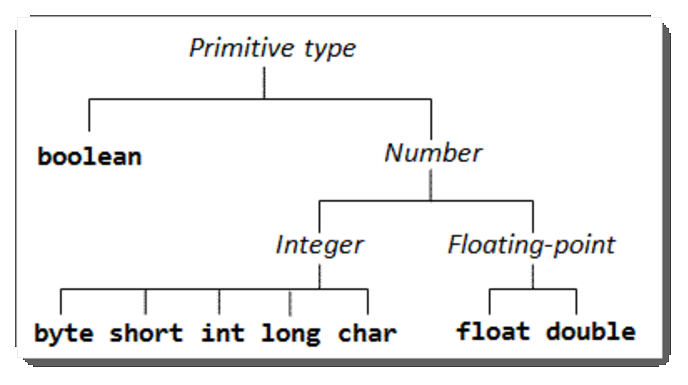
\includegraphics[width=.7\linewidth]{images/primitifs.pdf}
	\caption{Les types primitifs Java}
	\label{fig:typesprimitifs}
\end{figure}

\subsection{Les types primitifs numériques entiers}

Il existe 5 types primitifs entiers. Les 4 premiers représentent des nombres
entiers signés codés en notation en complément à 2. Il s'agit des types
: \pc{\bf byte}, \pc{\bf short}, \pc{\bf int} et \pc{\bf long}. 


La quantité mathématique montrée à la figure \vref{fig:7doigts} peut être
représentée de différentes manières : en utilisant des chiffres romains —~VII~—
ou arabes en base 10 —~7~— ou en base 2 —~111~— ou encore de moult autres
façons. 

Pour représenter un nombre négatif, l'habitude est de l'affubler du signe '-'
devant mais il est également possible d'utiliser la notation en complément à 2. 

\index{byte}
\index{short}
\index{int}
\index{long}
Les types \pc{byte}, \pc{short}, \pc{int} et \pc{long} représentent une partie
des nombres entiers signés. Ils sont stockés en notation en complément à 2. Ils
se différencient par la taille qu'ils occupent en mémoire et donc par
l'intervalle de nombres qu'ils représentent. 

La figure \vref{fig:typesbyteshortintlong} rassemble les types primitifs
entiers (excepté \pc{char}) avec leurs intervalles. 

\begin{figure}[h]
	\centering
	\begin{tabular}[h]{|l|l|p{9cm}|}
		\hline
		\rowcolor{black!20}
		\textbf{Type}	&	\textbf{Taille}	&	\textbf{Intervalle}	\\
		\hline
		\pc{byte}	&	8 bits	&	[-128, 127]\\
				&			&	[$-2^7$, $2^7-1$]\\
		\pc{short}	&	16 bits	&	[-32\,768-, 32\,767]\\
				&			&	[$-2^{15}$, $2^{15}-1$]\\
		\pc{int}		&	32 bits	&	[-2\,147\,483\,648, 2\,147\,483\,647]\\
				&			&	[$-2^{31}$, $2^{31}-1$]\\
		\pc{long}	&	64 bits	
			&	[-9\,223\,372\,036\,854\,775\,808, 9\,223\,372\,036\,854\,775\,807]\\
				&			&	[$-2^{63}$, $2^{63}-1$]\\
		\hline
	\end{tabular}	
	\caption{Types primitifs entiers (exceptés \pc{char}) et leur taille}
	\label{fig:typesbyteshortintlong}
\end{figure}

Le type \pc{int} est le type numérique entier privilégié. C'est celui qui est
le plus utilisé et est le type par défaut dans les opérations mathématiques
usuelles. L'intervalle qu'il représente est généralement suffisant%
\footnote{Ce qui n'est pas toujours vrai puisqu'en décembre 2014, la vidéo \textit{Gangnam Style} est la première vidéo Youtube à dépasser ±2 milliard de vues (2\,147\,483\,647 pour être précis) et oblique Google à revoir la variable dans laquelle elle stocke ce nombre de vues pour passer à 64 bits.}. 

\begin{figure}[h]
	\centering
	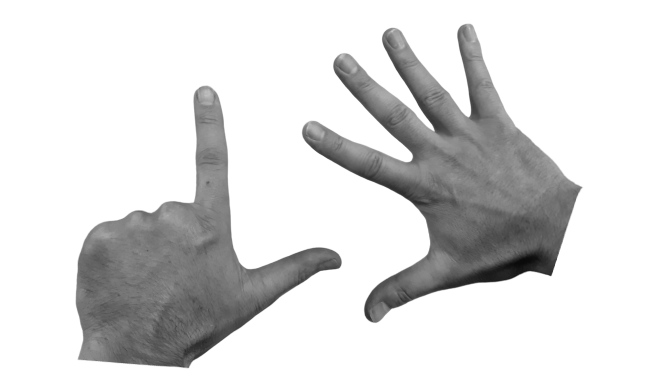
\includegraphics[width=.8\linewidth]{images/7doigts.png}
	\caption{La quantité 7 montrée avec les doigts}
	\label{fig:7doigts}
\end{figure}

\subsection{Les littéraux numérique entiers (excepté \pc{char})}

Les nombres entiers sont représentés en utilisant les chiffres habituels. Il
est cependant possible d'écrire un nombre dans différentes bases. Il faudra
alors pouvoir les distinguer. En mathématiques il est d'habitude d'utiliser un
indice pour préciser la base comme : $7_{10} = 111_2$. En informatique nous
utiliserons un \textbf{préfixe}.

\textbf{Littéral numérique décimal}

Respecte les règles suivantes~:

\begin{itemize}
	\item les chiffres \texttt{0123456789} et \texttt{\_};
	\item un littéral est de type \pc{int} ou \pc{long}, jamais de type 
		\pc{byte} ou \pc{short}\footnote{Ceci ne nous empêchera pas d'écrire 
		\pc{byte b = 5} par exemple. Nous verrons les conversions en 
		Développement II};
	\item pour distinguer un littéral \pc{long} du type par défaut \pc{int}, suffixer 
		d'un \texttt{l} ou \texttt{L};
\end{itemize}

\textit{Exemple, la quantité 100: }
\begin{java}
	int myInt = 100;
	int myOtherIntSomeValue = 1_00;
	long myLong = 100L;
\end{java}

\textbf{Littéral numérique octal}

Respecte les règles suivantes~:

\begin{itemize}
	\item les chiffres \texttt{01234567} et \texttt{\_};
	\item commence par un \texttt{0};
	\item un littéral est de type \pc{int} ou \pc{long}, jamais de type 
		\pc{byte} ou \pc{short};
	\item pour distinguer un littéral \pc{long} du type par défaut \pc{int}, suffixer 
		d'un \texttt{l} ou \texttt{L};
\end{itemize}

\textit{Exemple, la quantité 100: }
\begin{java}
	int myOctalInt = 0144;
	int anoherOctalInt = 01_44;
	long myOctalLong = 0144L;
\end{java}

\textbf{Littéral numérique hexadécimal}

Respecte les règles suivantes~:

\begin{itemize}
	\item les chiffres \texttt{0123456789ABCDEFabcdef} et \texttt{\_};
	\item commence par un \texttt{0x} ou \texttt{OX};
	\item un littéral est de type \pc{int} ou \pc{long}, jamais de type 
		\pc{byte} ou \pc{short};
	\item pour distinguer un littéral \pc{long} du type par défaut \pc{int}, suffixer 
		d'un \texttt{l} ou \texttt{L};
\end{itemize}

\textit{Exemple, la quantité 100: }
\begin{java}
	int myHexadecimalInt = 0x64;
	long myHexadecimalLong = 0X64l;
\end{java}

\clearpage
\textbf{Littéral numérique binaire}

Respecte les règles suivantes~:

\begin{itemize}
	\item les chiffres \texttt{01} et \texttt{\_};
	\item commence par un \texttt{0b} ou \texttt{OB};
	\item un littéral est de type \pc{int} ou \pc{long}, jamais de type 
		\pc{byte} ou \pc{short};
	\item pour distinguer un littéral \pc{long} du type par défaut \pc{int}, suffixer 
		d'un \texttt{l} ou \texttt{L};
\end{itemize}

\textit{Exemple, la quantité 100: } 
\begin{java}
	int myBinaryInt = 0b01100100;
	int anotherBinaryInt = 0B0110_0100;
\end{java}

\subsection{Le type primitif numérique entier particulier \pc{char}}

Le type \pc{char} est un entier non signé de 16~bits représentant le code 
Unicode codé en UTF-16 du caractère
	\footnote{%	
		Pour en savoir plus sur l'Unicode, UTF8, UTF16 et UTF32, lire
		«~Unicode, UTF8, UTF16, UTF32\ldots et tutti quanti~» \cite{pbt-unicode}
	}. 
Un caractère Unicode codé en UTF-16 fait une taille de 16 bits ou de 32 bits en
fonction du caractère qu'il représente. Le type \pc{char} en Java ne permet de
ne représenter que le sous ensemble BMP (\textit{Basic Multilingual Plane}) des
caractères Unicodes codés en UTF-16. Ceux ayant leur code compris entre
\texttt{\textbackslash u0000} et \texttt{\textbackslash uffff}. La figure 
\vref{fig:tableunicode} montre quelques caractères et leurs code Unicode. 

\begin{figure}[h]
	\centering
	\begin{tabular}[h]{|l|l|p{9cm}|}
		\hline
		\rowcolor{black!20}
		\textbf{Type}	&	\textbf{Taille}	&	\textbf{Intervalle}	\\
		\hline
		\pc{char}	&	16 bits	&	[0, 65\,535]\\
		&			&	[$0$, $2^{16}-1$]\\
		\hline
	\end{tabular}	
	\caption{Type primitif entier \pc{char} et sa taille}
	\label{fig:typeschar}
\end{figure}

\begin{figure}[t]
	\centering
	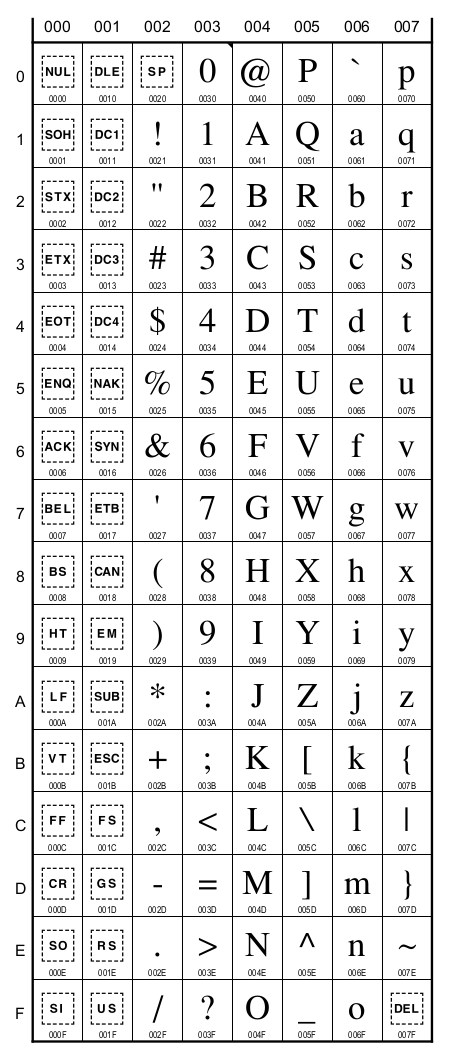
\includegraphics[width=.75\linewidth]{../images/unicode-latin-2.png}
	\caption{Table Unicode \textit{Basic Latin (ASCII)}}
	\label{fig:tableunicode}
\end{figure}

\subsection{Les littéraux numériques entiers \pc{char}}

Un littéral de type \pc{char} se caractérise par les guillemets simples
(\textit{single quote}) qui l'entourent. 

Le caractère \textit{a} par exemple, se représente \texttt{'a'}. Et l'on pourra
déclarer une variable de type \pc{char} et l'initialiser avec le caractère
\textit{a} par une instruction de la forme~:

\begin{java}
	char myChar = 'a';
\end{java}

La variable \pc{myChar} de type \pc{char} est initialisée avec le littéral
\pc{'a'} de type \pc{char} également. 


\clearpage
\marginicon{definition}
\index{séquence d'échappement}
À ceci s'ajoute la possibilité \textbf{d'échapper des caractères}. Un caractère
peut parfois avoir plusieurs significations. Par exemple le caractère
\textit{single quote} (\pc{'}) signale le début d'un littéral de type \pc{char}
mais peut vouloir signaler simplement le caractère~\pc{'}.   
Comment distinguer les deux ?

Lorsque l'on écrit simplement un caractère, il a sa signification habituelle~: 
\texttt{a} signifie \textit{a},
\texttt{b} signifie \textit{b},
\texttt{Z} signifie \textit{Z},
\texttt{'} signifie \textit{voici le début ou la fin d'un caractère}, etc. 
Certains caractères ont un \textbf{deuxième sens} lorsque qu'ils sont 
\textit{échappés}, c'est-à-dire précédés d'un \textit{backslash} 
(\pc{\textbackslash}). La figure \vref{tab:séquenceséchappements} montre les 
principaux.

\begin{figure}[h]
	\centering
	\begin{tabular}[h]{|l|p{6cm}|l|}
		\hline
		\rowcolor{black!20}
		\textbf{Caractère}	&	\textbf{Sens premier}	& \textbf{Sens second}	\\
		\hline
		n					&	n						& passage à la ligne	\\
		t					&	t						& tabulation		\\
		'					&	début ou fin d'un littéral \pc{char}	
														&	'	\\
		"					& 	début ou fin d'une chaine 	
														&	"	\\
		\textbackslash		& 	signale une séquence d'échappement 
								(ou \textit{attention, le caractère qui suit 
								n'a pas son sens premier}) 	
														&	\textbackslash	\\
		\hline
	\end{tabular}
	\caption{Quelques séquences d'échappement (la liste complète \cite{jls9} section 3.10.6)}
	\label{tab:séquenceséchappements}
\end{figure}



\subsection{Les types primitifs numériques à virgule flottante}

Les nombres pseudo-réels, ou encore les nombres à virgule flottante, sont un
sous ensemble des réels parce que —\,comme pour les entiers\,— il y aura un
\textit{plus petit nombre représentable} et \textit{un plus grand}. C'est
l'\textbf{intervalle} de nombre que l'on peut représenter. À ceci, s'ajoute la
\textbf{précision} que l'on pourra atteindre. En effet, les réels est un
ensemble continu de nombre —\,entre deux nombre réels, il existe toujours, au
moins, un autre réel\,— tandis que les pseudo-reéls est un ensemble discret. 

Les nombres à virgule flottante (\textit{floating numbers}) sont codés suivant
la norme \href{https://fr.wikipedia.org/wiki/IEEE_754}{IEEE\,754}. 

Selon cette norme, un nombre est représenté avec un signe, une mantisse et un
exposant. Le tout en base 2. Un bit est utilisé pour le signe.  

\[
	nombre = signe~mantisse_2~2^{exposant_2} 
\]

Il existe 2 types primitifs à virgule flottante~: \textbf{\texttt{float}} et
\textbf{\texttt{double}} dont les tailles sont données à la figure
\vref{fig:typefloat}.

\begin{figure}[h]
	\centering
	\begin{tabular}[t]{|l|c|c|c|}
		\hline
		\rowcolor{black!40}
		\textbf{Type} 	& \textbf{Taille (\textit{bit})}	
								& \textbf{Exposant} & \textbf{Mantisse}\\
		\hline
		float	& 32 bits					& 8		& 23\\
		\hline
		double	& 64 bits					& 11	& 52\\
		\hline
	\end{tabular}
	\caption{Types primitifs numériques à virgule flottante et leur taille}
	\label{fig:typefloat}
\end{figure}



\subsection{Les littéraux numériques à virgule flottante}

Les littéraux à virgule flottante sont composés de plusieurs parties~: une
partie entière, un point décimal (ou hexadécimal), une partie décimale, un
exposant et un suffixe.

\bigskip
\begin{center}
	\large\bf	| partie entière | . | partie décimale | exposant | suffixe |
\end{center}
\bigskip

Un littéral à virgule flottante peut être exprimé en base 10 (décimal) ou en 
base 16 (hexadécimal). 

Un littéral à virgule flottante est de type \pc{float} s'il est suffixé d'un
\pc{f} ou \pc{F} sinon, il est de type \pc{double}. Et ce qu'il soit suffixé
d'un \pc{d} ou \pc{D} ou non. 

Pour un \textbf{littéral décimal à virgule flottante}, au minimum un chiffre
dans la partie entière ou décimale et soit le point décimal, soit l'exposant,
soit le suffixe sont requis. Les autres parties sont optionnelles. 

\begin{itemize}

	\item la partie entière et la partie décimale sont des littéraux décimaux
		entiers (le caractère \pc{\_} étant autorisé);

	\item le point décimal est un point (\pc{.});

	\item l'exposant est la lettre \pc{e} ou \pc{E} suivie par un littéral
		décimal entier (le caractère \pc{\_} étant autorisé);

	\item le suffixe est \pc{f}, \pc{F}, \pc{d} ou \pc{D}

\end{itemize}

\textit{Exemples:}
\begin{java}
	double myDouble;
	myDouble = 1.;			// 1.0
	myDouble = .1;			// 0.1
	myDouble = 1e1;			// 10.0
	myDouble = 1d;			// 1.0
	myDouble = 1.e0;		// 1.0
	myDouble = 1_000.45;	// 1000.45
	myDouble = 1.45e3;		// 1450.0
	myDouble = .45e3d;		// 450.0
	
	float myFloat;
	myFloat = 1f;			// 1.0
	myFloat = 1.f			// 1.0	
\end{java}

Pour un \textbf{littéral hexadécimal à virgule flottante}, au minimum un
chiffre dans la partie entière ou décimale et l'exposant sont obligatoires. Le
suffixe est optionnel. 

\begin{itemize}

	\item le littéral débute par \pc{0x} ou \pc{0X};

	\item la partie entière et la partie décimale sont des chiffres hexadécimaux
		(le caractère \pc{\_} étant autorisé);

	\item le point décimal est un point (\pc{.});

	\item l'exposant est la lettre \pc{p} ou \pc{P} suivie par un littéral
	\marginicon{attention}
		décimal entier (le caractère \pc{\_} étant autorisé) représentant une 
		puissance de 2;

	\item le suffixe est \pc{f}, \pc{F}, \pc{d} ou \pc{D}

\end{itemize}

\textit{Exemples:}
\begin{java}
	double myDouble;
	myDouble = 0x1p0;		// 1.0 = 1 * 2^0
	myDouble = 0x1.1p0;	// 1.0625 = 1 + (1/16)
	myDouble = 0x1p1;		// 2.0 = 1 * 2^1
	myDouble = 0xA.Bp0; // 10.6875= 10 + 11*1/16
	myDouble = 0x1E2p2; // 1928 = (1*16^2 + 14*16^1 + 2*16^0) * 2^2

	float myFloat;
	myFloat = 0X.1p4f;		// 1.0 = (1*16^-1) * 2^4

\end{java}




\subsection{Le type primitif booléen}

Le type primitif booléen permet de représenter les deux valeurs logiques
\textit{vrai} et \textit{faux}. Ce sont les deux seules valeurs de ce type. 


\subsection{Les littéraux booléens}

Les littéraux booléens sont simplement~: \pc{true} pour \textit{vrai} et
\pc{false} pour \textit{faux}. 

\pagebreak[2]
\textit{Exemple:}
\nopagebreak
\begin{java}
	boolean myBoolean = true;
\end{java}










\index{type référence}
\section{Les types références}

Pour rappel (cfr. section \vref{primitif-reference}) une variable de type
référence est une variable qui ne contient pas directement la valeur qui lui
est assignée mais une référence vers cette valeur (qui se trouve à un autre
endroit).  

Tous les types qui ne sont pas un des 8 types primitifs présentés à la section
précédente sont des types références. Ce sont les types les plus répandus bien
que nous n'en verrons que quelques-uns dans ce premier cours de développement. 

Dans cette section, nous parlerons essentiellement de \texttt{String} et de
\textit{tableaux} bien que l'on ait déjà rencontré d'autres types références
comme \texttt{Scanner} ou \texttt{Random}. Pas d'inquiétude, nous leur règlerons
leur compte plus tard, en développement II. 

\clearpage
\subsection{Le type référence \texttt{String}}

\texttt{String} est un type référence. 

\begin{wrapfigure}{r}{.3\linewidth}
	\begin{center}
	\begin{tikzpicture}
		\node[draw, minimum width=.5cm, 
			minimum height=.5cm,label={above:\texttt{s}}] (ref) {};
		\node[draw, below of=ref, right] (string) at (0,0) {Hello};
		\draw[->] (ref.center) -- (string);
	\end{tikzpicture}
	\end{center}
\end{wrapfigure}

Pour rappel, déclarer une variable de type \texttt{String} a pour effet de
réserver un emplacement mémoire sur la pile (\textit{stack}). Initialiser cette
variable avec une valeur a pour effet de placer cette valeur sur le tas
(\textit{heap}). La variable \textit{référencera} cette valeur comme nous
pouvons le voir sur la figure ci-contre. 

La variable \texttt{s} se trouve sur la pile. 

La valeur \textit{"Hello"} se trouve sur le tas. 

Il est bien sûr possible de changer la valeur d'une variable de type référence,
et dans ce cas, c'est la référence qui change. Si la valeur initiale de
\texttt{s} est \textit{Hello} et qu'elle devient \textit{Bye bye}, la situation
sera par exemple comme illustré à la figure \vref{fig:hellobyebye}. Nous
y reviendrons. 

\begin{figure}[h]
	\centering
	\begin{tikzpicture}
		\node[draw, minimum width=.5cm, 
			minimum height=.5cm,label={above:\texttt{s}}] (ref) {};
		\node[draw, below of=ref, right] (string) at (0,0) {Hello};
		\node[draw, below of=string] (string2) at (3, 0) {Bye bye};
		\draw[->] (ref.center) -- (string2);
	\end{tikzpicture}
	\caption{Exemple : \texttt{s} reçoit \textit{Hello} et ensuite {Bye bye}}
	\label{fig:hellobyebye}
\end{figure}



\subsection{Les littéraux de type \texttt{String}}

Un littéral de type \texttt{String} se caractérise par les guillemets doubles
(\textit{double quote}) qui l'entourent (voir \cite{jls9} section 3.10.5). 

La chaine \textit{Hello} par exemple, se représente \texttt{"Hello"}. Et l'on
pourra déclarer une variable de type \texttt{String} et l'initialiser avec la
chaine \textit{Hello} par une instruction de la forme~:

\begin{java}
	String myString = "Hello";
\end{java}

Une chaine de caractères peut contenir n'importe quel caractère en ce compris,
des caractères d'échappement. La chaine \texttt{"Hello\textbackslash nWorld"}
a donc un sens et en cas d'affichage de cette chaine, nous verrons un passage
à la ligne entre \textit{Hello} et \textit{World}.  

Un littéral de type \texttt{String} donné —~par exemple
\texttt{"Hello"}~— référence toujours le même emplacement mémoire. Par exemple,
le code suivant s'illustre par la figure \vref{fig:somehello}. 

\begin{java}
	String s1 = "Hello";
	String s2 = "Hello";
\end{java}

\begin{figure}[h]
	\centering
	\begin{tikzpicture}
		\node[draw, minimum width=.5cm, 
			minimum height=.5cm,label={above:\texttt{s1}}] (ref1) {};
		\node[draw, minimum width=.5cm, 
			minimum height=.5cm,label={above:\texttt{s2}}] (ref2) at (1,0) {};
		\node[draw, below of=ref2, right] (string) at (2,-0.5) {Hello};
		\draw[->] (ref1.center) -- (string);
		\draw[->] (ref2.center) -- (string);
	\end{tikzpicture}
	\caption{Exemple : \texttt{s1} et \texttt{s2} reçoivent \textit{Hello}}
	\label{fig:somehello}
\end{figure}

\textbf{Remarque}~: ceci est vrai pour les littéraux de type \texttt{String}
pas pour des valeurs de type \texttt{String} qui seraient, par exemple, reçues
au \textit{runtime}. 

Le code suivant par exemple s'illustrerait par la figure
\vref{fig:differenthello}. 

\begin{java}
	Scanner keyboard = new Scanner(System.in);
	String s1 = keyboard.nextLine();	// INPUT Hello
	String s2 = keyboard.nextLine();	// INPUT Hello
\end{java}

\begin{figure}[h]
	\centering
	\begin{tikzpicture}
		\node[draw, minimum width=.5cm, 
			minimum height=.5cm,label={above:\texttt{s1}}] (ref1) {};
		\node[draw, minimum width=.5cm, 
			minimum height=.5cm,label={above:\texttt{s2}}] (ref2) at (1,0) {};
		\node[draw, below of=ref2, right] (string1) at (3,0) {Hello};
		\node[draw, below of=ref2, right] (string2) at (3,-1) {Hello};
		\draw[->] (ref1.center) -- (string2);
		\draw[->] (ref2.center) -- (string1);
	\end{tikzpicture}
	\caption{Exemple : \texttt{s1} et \texttt{s2} reçoivent \textit{Hello}}
	\label{fig:differenthello}
\end{figure}





\index{tableau}
\subsection{Les types références \textit{tableau}}

Les tableaux sont tous de types références. 

Pour rappel (cfr. section~\vref{chap:tableaux}), \textbf{déclarer} un
variable de type \textit{tableau de} a pour effet de réserver un emplacement
mémoire sur la pile (\textit{stack}). \textbf{Créer} le tableau réservera
l'emplacement mémoire sur le tas (\textit{heap}) et l'initialiser placera les
valeurs dans les cases du tableau comme illustré sur la figure \vref{fig:array1}. 

\begin{figure}[h]
	\centering
	\begin{tikzpicture}
		\node[draw, minimum width=.5cm, 
			minimum height=.5cm,label={above:\texttt{is}}] (ref1) {};
		\node[draw, minimum width=1cm,
			minimum height=1cm, below of=ref1, right] at (.5,-.5) (case1) {3};
		\node[draw, minimum width=1cm,
			minimum height=1cm, right of=case1]  (case2) {-14};
		\node[draw, minimum width=1cm,
			minimum height=1cm, right of=case2]  (case3) {15};
		\draw[->] (ref1.center) -- (case1);
	\end{tikzpicture}
	\caption{Exemple : \texttt{is} est un tableau de \texttt{int} (par exemple) ayant reçu les valeurs 3, -14 et 15 }
	\label{fig:array1}
\end{figure}

Il est bien sûr possible de changer la valeur d'un élément du tableau, voire
même de changer la valeur du tableau. 

% Déclaration
\begin{minipage}[t]{.5\linewidth}
	\textbf{Déclaration} du tableau \texttt{is}. 

	C'est un tableau d'entiers. Déclaré par~:
	\medskip
	\begin{java}
int[] is;
	\end{java}
\end{minipage}
\quad
\begin{minipage}[t]{.5\linewidth}
	\centering
	\vspace{.5cm}
	\begin{tikzpicture}
		\node[draw, minimum width=.5cm, 
			minimum height=.5cm,label={above:\texttt{is}}] (ref1) {};
	\end{tikzpicture}
\end{minipage}

\bigskip

% Création
\begin{minipage}[t]{.5\linewidth}
	\textbf{Création} du tableau d'entiers et \textbf{initialisation}. 
	La variable \texttt{is} contient une référence vers la mémoire qui contient
	le tableau.
	\medskip

	\begin{java}
int[] is = {3, -14, 15};
				
	\end{java}
\end{minipage}
\quad
\begin{minipage}[t]{.5\linewidth}
	\centering
	\vspace{.1cm}
	\begin{tikzpicture}
		\node[draw, minimum width=.5cm, 
			minimum height=.5cm,label={above:\texttt{is}}] (ref1) {};
		
		\node[draw, minimum width=1cm,
			minimum height=1cm, below of=ref1, right] at (.5,-.5) (case1) {3};
		\node[draw, minimum width=1cm,
			minimum height=1cm, right of=case1]  (case2) {-14};
		\node[draw, minimum width=1cm,
			minimum height=1cm, right of=case2]  (case3) {15};
		
		\draw[->] (ref1.center) .. controls(-1,-3) .. (case1);
	\end{tikzpicture}
\end{minipage}


\begin{minipage}[t]{.5\linewidth}
	\textbf{Remplacement} d'une valeur de type primitif dans le tableau. 
	La variable \texttt{is[1]}, de type primitif (\texttt{int}) reçoit directement
	une nouvelle valeur. 
	\medskip

	\begin{java}
int[] is = {3, -14, 15}
is[1] = 14;
	\end{java}
	\vspace{1cm}
\end{minipage}
\quad
\begin{minipage}[t]{.5\linewidth}
	\centering
	\vspace{.1cm}
	\begin{tikzpicture}
		\node[draw, minimum width=.5cm, 
			minimum height=.5cm,label={above:\texttt{is}}] (ref1) {};
		
		\node[draw, minimum width=1cm,
			minimum height=1cm, below of=ref1, right] at (.5,-.5) (case1) {3};
		\node[draw, minimum width=1cm,
			minimum height=1cm, right of=case1]  (case2) {\textbf{14}};
		\node[draw, minimum width=1cm,
			minimum height=1cm, right of=case2]  (case3) {15};
		
		\draw[->] (ref1.center) .. controls(-1,-3) .. (case1);
	\end{tikzpicture}
	\vspace{-2cm}
\end{minipage}

\bigskip

\begin{minipage}[t]{.5\linewidth}
	\textbf{Remplacement} du tableau par un autre tableau. 
	La variable \texttt{is}, de type référence (\texttt{int[]}), reçoit une 
	référence vers le nouveau tableau. 
	\medskip
	\begin{java}
int[] is = {3, -14, 15};
is[1] = 14;
is = new int[] {-2, 71, 82, 81};
	\end{java}
	\vspace{1cm}
\end{minipage}
\quad
\begin{minipage}[t]{.5\linewidth}
	\centering
	\vspace{.1cm}
	\begin{tikzpicture}
		\node[draw, minimum width=.5cm, 
			minimum height=.5cm,label={above:\texttt{is}}] (ref1) {};
		
		\node[draw, minimum width=1cm,
			minimum height=1cm, below of=ref1, right] at (.5,-.5) (case1) {3};
		\node[draw, minimum width=1cm,
			minimum height=1cm, right of=case1]  (case2) {14};
		\node[draw, minimum width=1cm,
			minimum height=1cm, right of=case2]  (case3) {15};
		
		\node[draw, minimum width=1cm,
			minimum height=1cm, below of=ref1, right] at (.5,-2.5) (case21) {-2};
		\node[draw, minimum width=1cm,
			minimum height=1cm, right of=case21]  (case22) {71};
		\node[draw, minimum width=1cm,
			minimum height=1cm, right of=case22]  (case23) {-82};
		\node[draw, minimum width=1cm,
			minimum height=1cm, right of=case23]  (case24) {81};
		\draw[->] (ref1.center) .. controls(-1,-3) .. (case21);
	\end{tikzpicture}
\end{minipage}



\subsection{Durée de vie des données sur le tas}

Les données de type référence sont créées sur le tas. Chaque fois que l'on crée
un tableau, une nouvelle chaine ou une nouvelle donnée de type référence, un
emplacement mémoire est réservé sur le tas pour contenir les valeurs. La
variable contiendra une référence vers ces valeurs. 

Nous avons vu qu'il était possible de changer la valeur d'une variable de type
référence. Dans ce cas, l'ancienne valeur n'est plus référencée. Lorsque plus
aucune variable ne référence une valeur en mémoire, elle n'est plus utile
à personne. Comment la récupérer pour libérer de l'espace mémoire qui, bien que
grand, n'est pas infini ?

Dans certains langages, c'est la tâche du développeur ou de la développeuse de
\textit{libérer} les emplacements mémoires qu'iel n'utilise plus. Dans d'autres
langages, c'est le langage qui s'en occupe. 

En langage Java, c'est le langage qui se charge de la gestion de la mémoire.
Lorsqu'il le décide, il lance un programme qui s'appelle le ramasse-miette
(\textit{garbage collector}\footnote{Notez que la traduction n'est pas
littérale.}) qui parcourt la mémoire à la recherche des valeurs non référencées
et rend les emplacements mémoires à nouveau disponibles. Il est possible de
demander explicitement le passage du ramasse-miette mais ce sera la machine
virtuelle qui décidera de son passage ou non. 






	
\renewcommand\bibname{Références}
\renewcommand\refname{your bibliography title}
\bibliographystyle{alpha} % Style des references: abbrv, plain, alpha...
\bibliography{../references}

\nocite{pbt-jdk7}
\nocite{pbt-jdk9}
%\nocite{test}


	% =======================================================
% Table des matières
% =======================================================
%\stopcontents[chapters]

\setcounter{tocdepth}{1}
\tableofcontents


\end{document}
